\stepcounter{Priloge}
\setcounter{equation}{0}
\setcounter{page}{1}
%%%%%%%%%%%%%%%%%%%%%%%%%%%%%%%%%%%%%%%%%%%%%%%%%%%%%%%%%%%%
\chapter{PROSTORSKE ROTACIJE}
\label{ch: Dodatek A}
\addcontentsline{loapp}{appendices}{A: PROSTORSKE ROTACIJE}
%%%%%%%%%%%%%%%%%%%%%%%%%%%%%%%%%%%%%%%%%%%%%%%%%%%%%%%%%%%%
\thispagestyle{fancy}

%Na tem mestu povzamemo dejstva o rotacijah in operacijah, povezanih z njimi, 
%ter izpeljave, ki jih potrebujemo v okviru tega dela. Ob�iren pregled podro�ja 
%rotacij je v svoji doktorski disertaciji predstavil Zupan \cite{ZupanPhd2003}. 
%Ker so rotacije pomemben del prostorskih problemov v mehaniki, jih obravnavajo 
%tudi v mnogih u�benikih in publikacijah (npr. Crisfield \cite{CrisfieldFE1997}, 
%Argyris \cite{Argyris1982}, Alturi in Cazzani \cite{AlturiCazzani1995}).


%-----------------------------------------------------------
\section{Rotacijska matrika}
\label{sec: Rotacijska matrika}
%-----------------------------------------------------------
V razdelku \ref{sec: Matematicni model} smo vpeljali prostorsko in telesno bazo 
prostora. Preslikava med obema ortonormiranima bazama, ki ju uporabljamo 
za opis prostorskega nosilca, je rotacija 
$R: \left\lbrace \bs{g}_{1}, \bs{g}_{2}, \bs{g}_{3} \right\rbrace
\longrightarrow \left\lbrace \bs{G}_{1}, \bs{G}_{2}, \bs{G}_{3} \right\rbrace$. 
V prostorski bazi lahko  rotaciji $R$ priredimo rotacijsko matriko 
$\bm{R}_g$, ki prostorsko bazo zavrti v telesno:
%
\begin{equation}
\bs{G}_{i,g} = \bm{R}_{g} \bs{g}_{i}.
\label{eq: rotacija baz}
\end{equation}
%
?e vektorje telesne baze $\bs{G}_{i,g}$, izra?ene v prostorski bazi, 
zapi?emo po komponentah
%
\begin{equation*}
\bs{G}_{i,g} = G_{g1,i}\bs{g}_{1} + G_{g2,i}\bs{g}_{2} + G_{g3,i}\bs{g}_{3}
, \quad i=1,2,3 ,
\end{equation*}
%
dobimo komponentni zapis rotacijske matrike. Njeni stolpci 
so komponente vektorjev telesne baze, izra?ene glede 
na prostorsko bazo: 
%
\begin{equation}
\bm{R}_{g} = \left[
\begin{array}{ccc}
G_{g1,1} & G_{g1,2} & G_{g1,3} \\
G_{g2,1} & G_{g2,2} & G_{g2,3} \\
G_{g3,1} & G_{g3,2} & G_{g3,3} 
\end{array} \right].
\end{equation}

Enako kot na baznih vektorjih deluje rotacijska matrika tudi 
na poljubnem vektorju v prostoru. Uporabljamo jo lahko
\begin{itemize}
\vspace*{-0.2cm}
\item[(i)] 	za rotacijo vektorja, 
			saj rotacijska matrika preslika poljuben vektor $\bs{v}_{g}$,  
			izra?en v prostorski bazi, v nov, zarotiran vektor 
			$\bs{w}_{g}$, izra?en v isti bazi
			\begin{equation*}
			\bs{w}_{g} = \bm{R}_{g} \bs{v}_{g},
			\end{equation*}
			ali
\vspace*{-0.1cm}
\item[(ii)] za koordinatno transformacijo. 
			Rotacijska matrika je namre? tudi prehodna matrika med 
			obema bazama, zato lahko komponente poljubnega vektorja 
			glede na prostorsko bazo izrazimo z njegovimi komponentami 
			glede na lokalno bazo:
			\begin{equation*}
			\bs{v}_{g} = \bm{R}_{g} \bs{v}_{G}.
			\end{equation*}
\end{itemize}

Podobno velja tudi za poljuben linearni operator $\mathcal{A}$. ?e 
mu v prostorski bazi pripada matrika $\bm{A}_{g}$, v telesni pa 
$\bm{A}_{G}$, je transformacija med obema zapisoma
\begin{equation}
\bm{A}_{g} = \bm{R}_{g} \bm{A}_{G}  \bm{R}_{g}^{T}.
\label{eq: transformacija matrike}
\end{equation}
%
Z uporabo pravila \eqref{eq: transformacija matrike} lahko poka?emo, 
da ima rotacijska matrika enak komponentni zapis v obeh bazah
\begin{equation*}
\bm{R}_{G} = \bm{R}_{g}^{T} \bm{R}_{g}  \bm{R}_{g} = \bm{R}_{g} = \bm{R},
\end{equation*}
zato indekse baz pri zapisu rotacijskih matrik v nadaljevanju izpu??amo.


Rotacijska matrika ima ?e naslednje lastnosti: 
%
\begin{itemize}
\vspace*{-0.3cm}
\item[(i)] rotacijska matrika $\bm{R}$ je ortogonalna matrika:
\begin{align}
&\bm{R}\bm{R}^{T}=\bm{R}^{T}\bm{R}=\bm{I}
\label{eq: rotacijska matrika je ortogonalna}, \\
&\bm{R}^{-1}=\bm{R}^{T},
\end{align}
kjer je $\bm{I}$ enotska matrika identi?ne preslikave
$I:\bs{a}\longrightarrow \bs{a}$;
\vspace*{-0.3cm}
\item[(ii)] ohranja dol?ino vektorja, na katerega deluje, in
\vspace*{-0.3cm}
\item[(iii)] ohranja kote med vektorji.
\end{itemize}
%


%-----------------------------------------------------------
\section{Kompozitum rotacij}
\label{sec: Kompozitum rotacij}
%-----------------------------------------------------------
Med tremi bazami v prostoru 
$\mathcal{B}_{g} : 
\left\lbrace \bs{g}_{1},\bs{g}_{2},\bs{g}_{3} \right\rbrace$, 
$\mathcal{B}_{G^{\left[ 1\right] }} : 
\left\lbrace \bs{G}_{1}^{\left[1\right]}\!,
\bs{G}_{2}^{\left[1\right]}\!,\bs{G}_{3}^{\left[1\right]}\right\rbrace$ 
in
$\mathcal{B}_{G^{\left[ 2\right] }} :
\left\lbrace \bs{G}_{1}^{\left[2\right]}\!,
\bs{G}_{2}^{\left[2\right]}\!,\bs{G}_{3}^{\left[2\right]}\right\rbrace$,
ki jih prikazuje slika \ref{fig: Kompozitum rotacij},
delujejo naslednje preslikave:
\begin{itemize}
\item[] $R^{\left[1\right]} : \mathcal{B}_{g}
\longrightarrow \mathcal{B}_{G^{\left[ 1\right] }} $, 
pripada ji rotacijska matrika $\bm{R}^{\left[1\right]}$,
\item[] $R^{\left[1-2\right]} : 
\mathcal{B}_{G^{\left[ 1\right] }}
\longrightarrow \mathcal{B}_{G^{\left[ 2\right] }} $, 
kateri pripada rotacijska matrika $\bm{R}^{\left[1-2\right]}$, in
\item[] $R^{\left[2\right]} : \mathcal{B}_{g}
\longrightarrow \mathcal{B}_{G^{\left[ 2\right] }}$, 
s pripadajo?o rotacijsko matriko  $\bm{R}^{\left[2\right]}$.
\end{itemize}
%
%
\begin{figure}[ht]
\begin{center}
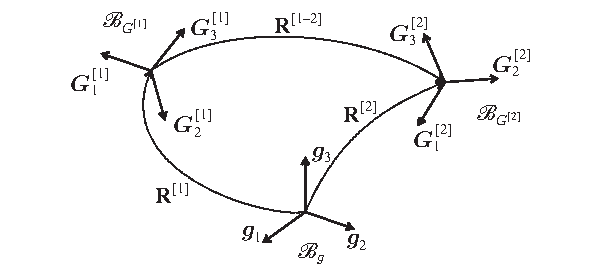
\includegraphics{Dodatki/slike/KompozitumRotacij}
\bicaption[fig: Kompozitum rotacij]{}{
Kompozitum rotacij.
}{Figure}{
Composition of rotations.}
\addfiguretolof{Composition of rotations.}
\end{center}
\end{figure}
%
%
Vektorje, izra?ene v posameznih bazah, lahko z rotacijskimi matrikami 
izrazimo v drugih bazah. Tako lahko na primer z rotacijsko matriko 
$\bm{R}^{\left[1-2\right]}$ 
poljuben vektor baze $\mathcal{B}_{G^{\left[ 2\right] }}$ izrazimo v bazi 
$\mathcal{B}_{G^{\left[ 1\right] }}$ kot 
$\bs{G}_{i}^{\left[2\right]} = \bm{R}^{\left[1-2\right]} 
\bs{G}_{i}^{\left[1\right]}$. Podobno 
bazni vektor $\bs{G}_{i}^{\left[1\right]}$ 
zapi?emo kot zavrten vektor $\bs{g}_{i}$ baze $\mathcal{B}_{g}$:
$\bs{G}_{i}^{\left[1\right]} = \bm{R}^{\left[1\right]} \bs{g}_{i}$.

?e zgornja zapisa zdru?imo, dobimo zvezo med baznimi vektorji baz 
$\mathcal{B}_{g}$ in $\mathcal{B}_{G^{\left[ 2\right] }}$:
\begin{equation*}
\bs{G}_{i}^{\left[2\right]} = \bm{R}^{\left[1-2\right]} \bm{R}^{\left[1\right]} \bs{g}_{i}.
\end{equation*}
%
Rotacijska matrika $\bm{R}^{\left[2\right]}$ je torej
\begin{equation}
\bm{R}^{\left[2\right]} = \bm{R}^{\left[1-2\right]} \bm{R}^{\left[1\right]}.
\label{eq: kompozitum rotacij}
\end{equation}
%
Za zdru?itev dveh rotaciji v eno samo moramo torej uporabiti 
operacijo mno?enja in ne se?tevanja, kar poudarimo tudi z izrazom 
`kompozitum rotacij'. Pokazali smo ?e, da ima rotacijska matrika 
enak komponentni zapis v bazah, med katerima slika, zato lahko tudi 
kompozitum rotacij v izrazu \eqref{eq: kompozitum rotacij} 
zapi?emo v eni od obeh baz:

\begin{equation*}
\bm{R}_{g}^{\left[2\right]} = \bm{R}_{g}^{\left[1-2\right]} \bm{R}_{g}^{\left[1\right]}
= \bm{R}_{G^{\left[2\right]}}^{\left[2\right]} = 
\bm{R}_{G^{\left[2\right]}}^{\left[1-2\right]} \bm{R}_{G^{\left[2\right]}}^{\left[1\right]}.
\end{equation*}

V primeru, da imamo rotacijsko matriko $\bm{R}^{\left[1-2\right]}$ 
izra?eno glede na bazo 
$\mathcal{B}_{G^{\left[ 1\right] }}$, dobi kompozitum rotacij 
\eqref{eq: kompozitum rotacij} z uporabo pravila \eqref{eq: transformacija matrike} 
naslednjo obliko:
\begin{equation}
\bm{R}_{g}^{\left[2\right]} = \bm{R}_{g}^{\left[1\right]} 
\bm{R}_{G^{\left[1\right]}}^{\left[1-2\right]}
\bm{R}_{g}^{\left[1\right]T} \bm{R}_{g}^{\left[1\right]}
 = \bm{R}_{g}^{\left[1\right]} 
 \bm{R}_{G^{\left[1\right]}}^{\left[1-2\right]}.
\label{eq: kompozitum rotacij v lokalni bazi}
\end{equation}
Pomembno je torej, da smo pri komponiranju rotacij pozorni na to, 
v katerih bazah so posamezne rotacijske matrike zapisane. Od tega je 
namre? odvisen vrstni red mno?enja rotacijskih matrik.


%-----------------------------------------------------------
\section{Parametrizacija rotacij}
\label{sec: Parametrizacija rotacij}
%-----------------------------------------------------------
Rotacijska matrika ima devet komponent, od katerih pa so  
zaradi lastnosti \eqref{eq: rotacijska matrika je ortogonalna} 
le tri med seboj neodvisne. 
Za izpeljavo ena?b nosilca je zato ugodneje uporabiti druga?en 
zapis rotacij. Med najpogosteje uporabljenimi je 
rotacijski vektor $\bs{\vartheta}$, ki je dolo?en s smerjo 
$\bs{n}$ in velikostjo rotacije $\vartheta$:
\begin{equation}
\bs{\vartheta} = \vartheta \bs{n}.
\end{equation}
%
?e vpeljemo anitisimetri?no matriko $\bm{S}\left(\bs{u} \right)$, 
ki pripada poljubnemu vektorju $\bs{u}$:
\begin{equation}
\bm{S}\left(\bs{u} \right) = 
\left[ 
\begin{array}{ccc}
0	 	 & -u_{3}	 & u_{2} \\
u_{3}	 & 0		 & -u_{1} \\
-u_{2}	 & u_{1}	 & 0 
\end{array}
\right] = -\bm{S}\left(\bs{u} \right)^{T},
\end{equation}
lahko rotacijsko matriko, parametrizirano z rotacijskim 
vektorjem, izrazimo z Rodriguesovo formulo \cite{Argyris1982,ZupanPhd2003}
\begin{equation}
\bm{R}\left(\bs{\vartheta} \right) = 
\bm{I}+\dfrac{\sin \vartheta}{\vartheta} 
\bm{S} \left( \bs{\vartheta}\right) +
\dfrac{1-\cos \vartheta}{\vartheta^2}
\bm{S}^2 \left( \bs{\vartheta}\right).
\label{eq: Rodriguesova formula}
\end{equation}
%
Pri tem je $\bm{I}$ identiteta in 
$\vartheta = \left\| \bs{\vartheta}\right\| =
\sqrt{\vartheta_{1}^{2} + \vartheta_{2}^{2} + 
\vartheta_{3}^{2}}$. 

Ob znani rotacijski matriki lahko njej pripadajo?i rotacijski vektor 
izra?unamo s Spurrierovim algoritmom \cite{Spurrier1978}. 
Ker je $\bs{\vartheta}$ lastni vektor matrike $\bm{R}$, velja
$\bs{\vartheta}_{g} = \bm{R}\bs{\vartheta}_{G} = \bs{\vartheta}_{G}$.

Za izpeljavo ena?b v okviru tega dela je smiselno vpeljati tudi 
operator $\bm{A}$, ki antisimetri?ni matriki priredi njen 
osni vektor $\bs{u}$
\begin{equation}
\bm{A}\left( \bm{S}\left( \bs{u}\right) \right) = \bs{u},
\end{equation}
%
in pripraviti nekaj zvez med antisimetri?nimi matrikami 
in njihovimi osnimi vektorji, ki izpeljave ena?b poenostavijo. 
Naj bosta $\bs{u}$ in $\bs{v}$ poljubna vektorja. Potem velja:
\begin{align}
\left(\bs{u} \cdot \bs{v}\right) 
\bm{S}\left(\bs{u}\right) &= 
-\bm{S}\left(\bs{u}\right) \bm{S}\left(\bs{v}\right) 
\bm{S}\left(\bs{u}\right)
\label{eq: lastnost antisimetricnih matrik 1}
\\
\bm{S}\left(\bs{u}\right)\bm{S}\left(\bs{v}\right)-
\bm{S}\left(\bs{v}\right)\bm{S}\left(\bs{u}\right) &=
\bm{S}\left( \bm{S}\left(\bs{u}\right) \bs{v} \right)
\label{eq: lastnost antisimetricnih matrik 2}
\\
\left(\bs{u} \cdot \bs{v}\right) \bm{S}\left(\bs{u}\right)
- \left(\bs{u} \cdot \bs{u}\right)\bm{S}\left(\bs{v}\right) &=
\bm{S}\left(\bm{S}^{2}\left(\bs{u}\right)\bs{v}\right).
\label{eq: lastnost antisimetricnih matrik 3}
\end{align}
%
Z antisimetri?nim operatorjem lahko nadomestimo tudi vektorski 
produkt dveh poljubnih vektorjev $\bs{u}$ in $\bs{v}$:
\begin{equation}
\bs{u}\times\bs{v} = \bm{S}\left(\bs{u}\right)\bs{v} = 
- \bm{S}\left(\bs{v}\right)\bs{u}.
\label{eq: vektorski produkt izrazen z antisimetricno matriko}
\end{equation}
%
Iz identitete 
$\bm{S}\left( \bs{u}\right) = \bm{R}^{T}\bm{S}\left( \bs{v}\right) \bm{R}$ sledi
\begin{equation}
\bs{u} = \bm{R}^{T} \bs{v}.
\label{eq: relacija u v}
\end{equation}


%-----------------------------------------------------------
\section{Variacija rotacijske matrike, parametrizirane 
			z rotacijskim vektorjem}
\label{sec: Variacija rot vektor}
%-----------------------------------------------------------
Variacijo rotacijskega operatorja lahko v na�em primeru izra?unamo s smernim odvodom. 
Pri tem upo?tevamo 
definicijo smernega odvoda, ki pravi, da je smerni odvod rotacije limita z 		
$\epsilon\delta\bs{\vartheta}$ povzro?ene spremembe operatorja $\bm{R}$, ko gre 
$\epsilon$ proti ni?. Rotacija, ki pripada spremembi 
rotacijskega vektorja $\epsilon\delta\bs{\vartheta}$, je enaka
$\bm{R(\epsilon\delta\bs{\vartheta})}$, skupna rotacija pa je kompozitum trenutne 
rotacije in njene spremembe:
$\bm{R(\epsilon\delta\bs{\vartheta})}\bm{R(\vartheta)}$.
%

Smerni odvod rotacijske matrike torej izra?unamo kot
\begin{equation*}
\delta \bm{R}\left(\bs{\vartheta} \right) = 
\dfrac{d}{d\epsilon}\bigg|_{\epsilon=0} 
\bm{R}\left( \epsilon\delta \bs{\vartheta} \right) 
\bm{R}\left( \bs{\vartheta}\right) .
\end{equation*}
%
$\bm{R}\left( \epsilon\delta\vartheta \right)$ zapi?emo z 
Rodriguesovo formulo \eqref{eq: Rodriguesova formula},
 odvajamo po $\epsilon$, izvrednotimo 
pri $\epsilon = 0$ in dobimo:
\begin{equation}
\delta \bm{R}\left(\bs{\vartheta} \right) =
\bm{S}\left( \delta \bs{\vartheta}\right) 
\bm{R}\left(\bs{\vartheta} \right) .
\end{equation}
%
Sprememba rotacije pa je lahko dolo?ena tudi kot komponiranje z 
desne $\bm{R}\left(\bs{\vartheta}_{g}\right) 
\bm{R}\left(\epsilon\delta\bs{\vartheta}_{G}\right)$ 
(v tem zapisu smo z indeksom $g$ poudarili, da gre za bazo $\mathcal{B}_{g}$, 
v nadaljevanju izpeljave pa $g$ pri $\vartheta$ opu??amo).
Sledi
\begin{equation}
\delta \bm{R}\left(\bs{\vartheta} \right) =
\bm{R}\left(\bs{\vartheta} \right)
\bm{S}\left( \delta \bs{\vartheta}_{G}\right) . 
\label{eq: odvod rotacije z desne}
\end{equation}
%
Ker morata biti variaciji obeh izrazov enaki, velja
\begin{equation}
\bm{S}\left( \delta \bs{\vartheta}_{G}\right) = 
\bm{R}^{T} \bm{S}\left( \delta \bs{\vartheta}_{g}\right) \bm{R}.
\end{equation}
%
Od tod in iz ena�be \eqref{eq: relacija u v} je potem
\begin{equation}
\delta \bs{\vartheta}_{G} = \bm{R}^{T} \delta \bs{\vartheta}_{g}.
\end{equation}

V ena?bah nosilca variacija rotacijske matrike ve?krat deluje 
na vektorju. Ob upo?tevanju ena?be 
\eqref{eq: vektorski produkt izrazen z antisimetricno matriko} izpeljemo
\begin{equation}
\delta \bm{R}\left( \bs{\vartheta} \right) \bs{u} = 
\bm{S} \left( \delta \bs{\vartheta} \right) 
\bm{R}\left( \bs{\vartheta} \right) \bs{u} = 
\delta \bs{\vartheta} \times \bm{R}\left( \bs{\vartheta} \right) \bs{u} = 
- \bm{R}\left( \bs{\vartheta} \right) \bs{u} \times \delta \bs{\vartheta} = 
- \bm{S} \left( \bm{R}\left( \bs{\vartheta} \right) \bs{u}\right) 
\delta \bs{\vartheta}. 
\label{eq: variacija rotacije na vektorju neaditivno}
\end{equation}
%
Variacijo rotacijske matrike, ki deluje na poljubnem vektorju $\bs{u}$, 
lahko torej izrazimo z variacijo rotacijskega vektorja.


%-----------------------------------------------------------
\section{Variacija rotacijske matrike, parametrizirane 
				z aditivnim rotacijskim vektorjem}
\label{sec: Variacija adititvni rot vektor}
%-----------------------------------------------------------
V primeru meh?anja materiala so glede na izbrani opis 
deformacij \eqref{eq: deformacijski nastavek za game} in 
\eqref{eq: deformacijski nastavek za kape} funkcije kinemati?nih koli?in 
izra?ene z zveznim in nezveznim delom. Slednji je zapisan v telesni bazi prostora, zato se 
sre?amo z rotacijskimi matrikami, parametriziranimi z rotacijskim vektorjem, ki je zapisan 
v telesni bazi prostora: $\bm{R} \left( \bs{\vartheta}_G \right)$. Njihove spremembe 
dolo?amo s komponiranjem z desne, smerni odvod pa z izrazom
\begin{equation}
\delta \bm{R}\left(\bs{\vartheta}_G \right) = 
\dfrac{d}{d\epsilon}\bigg|_{\epsilon=0} 
\bm{R}\left( \bs{\vartheta}_G \right)
\bm{R}\left( \epsilon\delta \bs{\vartheta}_G \right).
\end{equation}

%
Rotacijo $\bm{R}\left( \epsilon\delta \bs{\vartheta}_G \right)$, ki pripada spremembi 
rotacijskega vektorja $\epsilon\delta \bs{\vartheta}_G$, zapi?emo z Rodriguesovo formulo 
\eqref{eq: Rodriguesova formula}, odvajamo po $\epsilon$ in izvrednotimo pri $\epsilon=0$. 
Tako dobimo:
\begin{equation}
\delta \bm{R}\left(\bs{\vartheta}_G \right) = 
\bm{R}\left( \bs{\vartheta}_G \right)
\bm{S}\left( \delta \bs{\vartheta}_G \right).
\label{eq: variacija rotacije pri komponiranju z desne}
\end{equation}

Spremenjeno rotacijsko matriko pa lahko opi?emo tudi tako, 
da rotacijskemu vektorju spremembo kar pri?tejemo: 
$\bm{R}\left(\bs{\vartheta}_{G} + 
\epsilon\delta\bs{\vartheta}_{G}^{A} \right)$. Pri tem je 
$\delta\bs{\vartheta}_{G}^{A}$ tako imenovani `aditivni' 
rotacijski vektor, dolo?imo pa ga tako, da velja
\begin{equation}
\delta \bm{R}\left(\bs{\vartheta}_{G}\right)  = 
\dfrac{d}{d\epsilon}\bigg|_{\epsilon=0} 
\bm{R}\left(\bs{\vartheta}_{G} + 
\epsilon\delta\bs{\vartheta}_{G}^{A} \right).
\end{equation}
%
$\bm{R}\left(\bs{\vartheta}_{G} + 
\epsilon\delta\bs{\vartheta}_{G}^{A} \right)$ 
zapi?emo z Rodriguesovo formulo \eqref{eq: Rodriguesova formula}, 
odvajamo po $\epsilon$ in izvrednotimo pri $\epsilon=0$:
\begin{align}
\delta \bm{R}\left(\bs{\vartheta}_{G}\right)  = & \,
\dfrac{\sin \vartheta}{\vartheta}\bm{S}\left( \delta\bs{\vartheta}_{G}^{A}\right) 
+ \dfrac{1-\cos\vartheta}{\vartheta^2}
\left( 
\bm{S}\left( \delta\bs{\vartheta}_{G}^{A}\right) \bm{S}\left( \bs{\vartheta}_{G}\right)
+ \bm{S}\left( \bs{\vartheta}_{G}\right) \bm{S}\left( \delta\bs{\vartheta}_{G}^{A}\right)
\right) \notag\\
&+ \dfrac{\vartheta \cos \vartheta - \sin \vartheta}{\vartheta^3}
\left( 
\bs{\vartheta}_{G} \cdot \delta\bs{\vartheta}_{G}^{A}
\right) \bm{S}\left( \bs{\vartheta}_{G} \right)  \notag \\
&+ \dfrac{\vartheta \sin \vartheta - 2\left( 1-\cos \vartheta\right) }{\vartheta^4}
\left( 
\bs{\vartheta}_{G} \cdot \delta\bs{\vartheta}_{G}^{A}
\right) \bm{S}^2\left( \bs{\vartheta}_{G} \right).
\label{eq: variacija rotacijske matrike aditivno}
\end{align}
%
Za variacijo rotacijske matrike v smislu aditivnega rotacijskega vektorja 
lahko z upo?tevanjem lastnosti \eqref{eq: rotacijska matrika je ortogonalna} 
poka?emo, da je produkt 
$\delta \bm{R}\bm{R}^{T}$ antisimetri?na matrika
\begin{equation*}
\bm{R}\bm{R}^{T} = \bm{I} \qquad \Rightarrow \qquad
\delta \bm{R}\bm{R}^{T} + \bm{R} \delta \bm{R}^{T} = 0 
\qquad \Rightarrow \qquad
\delta \bm{R}\bm{R}^{T} =- \bm{R} \delta \bm{R}^{T} = 
- \left( \delta \bm{R}\bm{R}^{T}\right) ^{T} .
\end{equation*}
%
?e sedaj izraz \eqref{eq: variacija rotacijske matrike aditivno} z desne 
pomno?imo z $\bm{R}^{T}\left( \bs{\vartheta}_{G}\right) $ in upo?tevamo 
anitisimetri?nost produkta $\delta \bm{R}\bm{R}^{T}$, 
dobimo po kon?anem urejanju
\begin{equation}
\delta \bm{R}\left(\bs{\vartheta}_{G}\right) 
\bm{R}^{T}\left(\bs{\vartheta}_{G}\right) = 
\bm{S} 
\left(
\delta \bs{\vartheta}_{G}^{A}+ 
\dfrac{1-\cos\vartheta}{\vartheta^2}\bm{S}\left( \bs{\vartheta}_{G} \right)
\delta \bs{\vartheta}_{G}^{A} + 
\dfrac{\vartheta-\sin\vartheta}{\vartheta^3}
\bm{S}^2\left( \bs{\vartheta}_{G} \right)\delta \bs{\vartheta}_{G}^{A}
\right) ,
\end{equation}
pri ?emer lahko na desni strani izraza prepoznamo produkt transformacijske 
matrike $\bm{T}\left( \bs{\vartheta}_{G}\right) $ 
\begin{equation}
\bm{T}\left( \bs{\vartheta}\right) = 
\bm{I} + \dfrac{1-\cos\vartheta}{\vartheta^2} \bm{S}\left( \bs{\vartheta}\right) + 
\dfrac{\vartheta-\sin\vartheta}{\vartheta^3} \bm{S}^2\left( \bs{\vartheta}\right)
\label{eq: transformacijska matrika}
\end{equation}
%
in aditivne variacije 
$\delta \bs{\vartheta}_{G}^{A}$. Potem je
\begin{equation}
\delta \bm{R}\left(\bs{\vartheta}_{G}\right) 
\bm{R}^{T}\left(\bs{\vartheta}_{G}\right) = 
\bm{S} 
\left(
\bm{T}\left( \bs{\vartheta}_{G}\right)
\delta \bs{\vartheta}_{G}^{A}
\right) .
\label{eq: variacija v smislu aditivnega vektorja}
\end{equation}
%
Izraz \eqref{eq: variacija v smislu aditivnega vektorja} lahko sedaj 
primerjamo z izrazom \eqref{eq: variacija rotacije pri komponiranju z desne}, ki ga z desne 
pomno?imo z $\bm{R}^{T}\left( \bs{\vartheta}_{G}\right) $. Tako dobimo
povezavo med aditivno variacijo $\delta \bs{\vartheta}_{G}^{A}$ in
multiplikativno variacijo $\delta \bs{\vartheta}_{G}$:
\begin{equation}
\delta \bs{\vartheta}_{G} = 
\bm{R}^{T}\left(\bs{\vartheta}_{G}\right) 
\bm{T}\left( \bs{\vartheta}_{G}\right)
\delta \bs{\vartheta}_{G}^{A} = 
\bm{T}^{T}\left( \bs{\vartheta}_{G}\right)
\delta \bs{\vartheta}_{G}^{A}.
\label{eq: aditivna - multiplikativna variacija}
\end{equation}
%
Pri tem smo upo?tevali zvezo $\bm{R}^{T} \bm{T} = \bm{T}^{T}$.

Tudi variacijo rotacijske matrike v smislu aditivnega rotacijskega vektorja 
$\delta \bm{R}\left( \bs{\vartheta}_{G}\right) $, ki deluje na 
poljubnem vektorju $\bs{u}$, je zaradi re?evanja ena?b koristno 
izraziti z variacijo aditivnega rotacijskega vektorja. 
Izraz \eqref{eq: variacija rotacije pri komponiranju z desne} najprej 
pomno?imo z $\bs{u}$, upo?tevamo 
\eqref{eq: aditivna - multiplikativna v
\begin{align}
\delta \bm{R} \left( \bs{\vartheta}_{G}\right) \bs{u} &= 
\bm{R} \left( \bs{\vartheta}_{G}\right) 
\bm{S} \left( \delta \bs{\vartheta}_{G}\right) \bs{u} \notag \\
&= -\bm{R} \left( \bs{\vartheta}_{G}\right)
\bm{S} \left( \bs{u}\right) \delta \bs{\vartheta}_{G} \notag \\
&= -\bm{R} \left( \bs{\vartheta}_{G}\right)
\bm{S} \left( \bs{u}\right)\bm{T}^{T}\left( \bs{\vartheta}_{G}\right)
\delta \bs{\vartheta}_{G}^{A}.
\label{eq: variacija rotacije na vektorju aditivno}
\end{align}
